\documentclass[
	10pt,								% globale Schriftgröße
	parskip=half-,						% setzt Absatzabstand hoch
	paper=a4,							% Format
	english,ngerman,					% lädt Sprachpakete
	]{scrartcl}							% Dokumentenklasse

% //////////////////// Pakete laden ////////////////////
\usepackage[fleqn]{amsmath}
\usepackage[fleqn]{mathtools}
\usepackage{amssymb}			% mathematische symbole, für \ceckmarks
\usepackage{amsthm}				% für proof
\usepackage{mathrsfs}			% für \mathscr
\usepackage{latexsym}
\usepackage{marvosym}				% für Lightning

\usepackage{fontspec} 			% funktioniert nur mit den neueren Compilern z.B. XeLaTeX
\usepackage{microtype}			% für bessere Worttrennung
\usepackage[ngerman]{babel} 	% Spracheinstellung
\usepackage{lmodern}			% verändert verwendete Schriftart, damit sie weniger pixelig ist

\usepackage{verbatim}
\usepackage{listings}			% Für Quellcode

\usepackage{graphicx}
\usepackage{tabularx}			% für Tabellen mit gleicher Spaltenbreite und automatischen Umbrüchen
\usepackage{fullpage}
\usepackage{multirow}			% für multirow in tabulars
\usepackage{rotate}
\usepackage[cmyk,table]{xcolor} % um Farben zu benutzen, kann mehr als das Paket color
\usepackage[					% Verlinkungen
	colorlinks,					% farbige Schrift, statt farbiger Rahmen
	linktocpage,				% verlinkt im Abb.Verzeichnis Seitenzahl statt Bildunterschrift
	linkcolor=blue				% setzt Farbe der Links auf blau
	]{hyperref}					% nur für digitale Anwendungen, url = "http://www.example.com"
\usepackage{url}				% für Webadressen wie e-mail usw.: "\url{http://www.example.com}"

\usepackage{enumerate}			% für versch. Aufzählungezeichen wie z.B. a)
\usepackage{xspace}				% folgt ein Leerzeichen nach einem \Befehl, wird es nicht verschluckt.
\usepackage{cancel}				% für das Durchstreichen u.a. in Matheformeln mit \cancel
\usepackage{float}              % zum Forcieren der Position von figure-Umgebungen

% zum Zeichnen (u.a. von Graphen)
\usepackage{fp}
\usepackage{tikz}
\usetikzlibrary{tikzmark}			% für \tikzmark{toRemember}
\usetikzlibrary{positioning}	% verbesserte Positionierung der Knoten
\usetikzlibrary{automata}		% für Automaten (GTI)
\usetikzlibrary{arrows}
\usetikzlibrary{shapes}
\usetikzlibrary{decorations.pathmorphing}
\usetikzlibrary{decorations.pathreplacing}
\usetikzlibrary{decorations.shapes}
\usetikzlibrary{decorations.text}

% //////////////////// Syntaxhighlighting ////////////////////
\lstloadlanguages{Python, Haskell, [LaTeX]TeX, Java}
\lstset{
   basicstyle=\footnotesize\ttfamily,	% \scriptsize the size of the fonts that are used for the code
   backgroundcolor = \color{bgcolour},	% legt Farbe der Box fest
   breakatwhitespace=false,	% sets if automatic breaks should only happen at whitespace
   breaklines=true,			% sets automatic line breaking
   captionpos=t,				% sets the caption-position to bottom, t for top
   commentstyle=\color{codeblue}\ttfamily,% comment style
   frame=single,				% adds a frame around the code
   keepspaces=true,			% keeps spaces in text, useful for keeping indentation
							% of code (possibly needs columns=flexible)
   keywordstyle=\bfseries\ttfamily\color{codepurple},% keyword style
   numbers=left,				% where to put the line-numbers;
   							% possible values are (none, left, right)
   numberstyle=\tiny\color{codegreen},	% the style that is used for the line-numbers
   numbersep=5pt,			% how far the line-numbers are from the code
   stepnumber=1,				% nummeriert nur jede i-te Zeile
   showspaces=false,			% show spaces everywhere adding particular underscores;
							% it overrides 'showstringspaces'
   showstringspaces=false,	% underline spaces within strings only
   showtabs=false,			% show tabs within strings adding particular underscores
   flexiblecolumns=false,
   tabsize=1,				% the step between two line-numbers. If 1: each line will be numbered
   stringstyle=\color{orange}\ttfamily,	% string literal style
   numberblanklines=false,				% leere Zeilen werden nicht mitnummeriert
   xleftmargin=1.2em,					% Abstand zum linken Layoutrand
   xrightmargin=0.4em,					% Abstand zum rechten Layoutrand
   aboveskip=2ex, 
}

\lstdefinestyle{py}{
   language=Python,
}
\lstdefinestyle{hs}{
   language=Haskell,
}
\lstdefinestyle{tex}{
	language=[LaTeX]TeX,
	escapeinside={\%*}{*)},     % if you want to add LaTeX within your code
	texcsstyle=*\bfseries\color{blue},% hervorhebung der tex-Schlüsselwörter
	morekeywords={*,$,\{,\},\[,\],lstinputlisting,includegraphics,
	rowcolor,columncolor,listoffigures,lstlistoflistings,
	subsection,subsubsection,textcolor,tableofcontents,colorbox,
	fcolorbox,definecolor,cellcolor,url,linktocpage,subtitle,
	subject,maketitle,usetikzlibrary,node,path,addbibresource,
	printbibliography},% if you want to add more keywords to the set
     numbers=none,
     numbersep=0pt,
     xleftmargin=0.4em,
}

\lstdefinestyle{java}{
	language=Java,
	extendedchars=true,		% lets you use non-ASCII characters;
   						% for 8-bits encodings only, does not work with UTF-8
}

\lstdefinelanguage[x64]{Assembler}     % add a "x64" dialect of Assembler
   [x86masm]{Assembler} % based on the "x86masm" dialect
   % with these extra keywords:
   {morekeywords={CDQE,CQO,CMPSQ,CMPXCHG16B,JRCXZ,LODSQ,MOVSXD, %
                  POPFQ,PUSHFQ,SCASQ,STOSQ,IRETQ,RDTSCP,SWAPGS, %
                  rax,rdx,rcx,rbx,rsi,rdi,rsp,rbp, %
                  r8,r8d,r8w,r8b,r9,r9d,r9w,r9b}
}					% for 8-bits encodings only, does not work with UTF-8

\lstdefinestyle{c}{
	language=c,
	extendedchars=true,		% for 8-bits encodings only, does not work with UTF-8
}

% //////////////////// eigene Kommandos ////////////////////
\newcommand\FU{Freie Universität Berlin\xspace}% benötigt package xspace
\newcommand\gdw{g.\,d.\,w.\xspace}
\newcommand\oBdA{o.\,B.\,d.\,A.\xspace}
\newcommand{\Eu}{\texteuro}
\newcommand\N{\mathbb{N}\xspace}
\newcommand\Q{\mathbb{Q}\xspace}
\newcommand\R{\mathbb{R}\xspace}
\newcommand\Z{\mathbb{Z}\xspace}
\newcommand\ohneNull{\ensuremath{\backslash\lbrace 0\rbrace}}% \{0}
\let\dhALT\dh	% Schreibt Befehl \dh in \dhALT um
\renewcommand\dh{d.\,h.\xspace}	%renew überschreibt command \dh
\newcommand\Bolt{\;\text{\LARGE\raisebox{-0.3em}{\Lightning}\normalsize}\xspace}% Blitz
\newcommand\zz{\ensuremath{\raisebox{+0.25ex}{Z}% zu zeigen
			\kern-0.4em\raisebox{-0.25ex}{Z}%
			\;\xspace}}
\newcommand{\from}{\ensuremath{\colon}}
\newcommand{\floor}[1]{\lfloor{#1}\rfloor}
\newcommand{\ceil}[1]{\lceil{#1}\rceil}
 \renewcommand{\L}{\ensuremath{\mathcal{L}}\xspace}
 \renewcommand{\P}{\ensuremath{\mathcal{P}}\xspace}
 \newcommand{\NL}{\ensuremath{\mathcal{N}\kern-0.2em\mathcal{L}}\xspace}
 \newcommand{\NP}{\ensuremath{\mathcal{NP}}\xspace}

% //////////////////// Mathefunktionen ////////////////////
\DeclareMathOperator{\Landau}{\mathcal{O}}
\DeclareMathOperator{\True}{True}
\DeclareMathOperator{\False}{False}

% //////////////////// eigene Theoreme ////////////////////
\newtheorem{theorem}{Satz}
\newtheorem{corollary}[theorem]{Folgerung}
\newtheorem{lemma}[theorem]{Lemma}
\newtheorem{observation}[theorem]{Beobachtung}
\newtheorem{definition}[theorem]{Definition}
\newtheorem{Literatur}[theorem]{Literatur}
% konfiguriert proof
\makeatletter
\newenvironment{Proof}[1][\proofname]{\par
  \pushQED{\qed}%
  \normalfont \topsep6\p@\@plus6\p@\relax
  \trivlist
  \item[\hskip\labelsep
%         \itshape
        \bfseries
    #1\@addpunct{.}]\ignorespaces
}{%
  \popQED\endtrivlist\@endpefalse
}
\makeatother

% //////////////////// eigene Farben ////////////////////
\let\definecolor=\xdefinecolor
\definecolor{FUgreen}{RGB}{153,204,0}
\definecolor{FUblue}{RGB}{0,51,102}

\definecolor{middlegray}{rgb}{0.5,0.5,0.5}
\definecolor{lightgray}{rgb}{0.8,0.8,0.8}
\definecolor{orange}{rgb}{0.8,0.3,0.3}
\definecolor{azur}{rgb}{0,0.7,1}
\definecolor{yac}{rgb}{0.6,0.6,0.1}
\definecolor{Pink}{rgb}{1,0,0.6}

\definecolor{bgcolour}{rgb}{0.97,0.97,0.97}
\definecolor{codegreen}{rgb}{0,0.6,0}
\definecolor{codegray}{rgb}{0.35,0.35,0.35}
\definecolor{codepurple}{rgb}{0.58,0,0.82}
\definecolor{codeblue}{rgb}{0.4,0.5,1}

% //////////////////// eigene Settings ////////////////////

\textheight = 230mm		% Höhe des Satzspiegels / Layouts
\footskip = 10ex			% Abstand zw. Fußzeile und Grundlinie letzter Textzeile
\parindent 0pt			% verhindert Einrückung der 1. Zeile eines Absatzes
\setkomafont{sectioning}{\rmfamily\bfseries}% setzt Ü-Schriften in Serifen, {disposition}											% bindet Header ein (WICHTIG)
\usepackage{graphicx}
\usepackage{amsmath}
\usepackage{amssymb}
\usepackage{fancyvrb}

\newcommand{\dozent}{Prof. R. Rojas}					% <-- Names des Dozenten eintragen
\newcommand{\projectNo}{10}
\newcommand{\veranstaltung}{Mustererkennung}
\newcommand{\semester}{WS17/18}
\newcommand{\studenten}{Boyan Hristov, Nedeltscho Petrov}
% /////////////////////// BEGIN DOKUMENT /////////////////////////


\begin{document}
% /////////////////////// BEGIN TITLEPAGE /////////////////////////
\begin{titlepage}
	\subject{\dozent}
	\title{\veranstaltung, \semester}
	\subtitle{\Large Übungsblatt \projectNo\\ \large\vspace{1ex} }
	\author{\studenten}
	\date{\normalsize \today}
\end{titlepage}

\maketitle								% Erstellt das Titelblatt
\vspace*{-9cm}							% rückt Logo an den oberen Seitenrand
\makebox[\dimexpr\textwidth+1cm][r]{	%rechtsbündig und geht rechts 1cm über Layout hinaus
	
\includegraphics[width=0.4\textwidth]{src/fu_logo} % fügt FU-Logo ein
}
% /////////////////////// END TITLEPAGE /////////////////////////

\vspace{7cm}							% Abstand
\rule{\linewidth}{0.8pt}				% horizontale Linie										% erstellt die Titelseite


Link zum Git Repository: \url{https://github.com/BoyanH/FU-MachineLearning-17-18/tree/master/Solutions/Homework\projectNo}

\section*{Ada Boost und Face Detection}


\section*{Dataset}

\begin{lstlisting}
\item MIT-CBCL-database
\item Link: \url{https://github.com/HyTruongSon/Pattern-Classification/tree/master/MIT-CBCL-database}
\item Training set - 2 429 Bilder mit Gesichter, 4 548 ohne
\item Test set - 472 Bilder mit Gesichter, 23 573 ohne
\end{lstlisting}

Der Datensatz hat leider wenigere Bilder mit Gesichter. Das ist im Testfall ganz gut, beim Trainieren aber
eher unausreichend. Man könnte theoretisch beim Trainieren noch weitere Daten, z.B. von dem Gesichtsdatensatz aus
der vorherigen Hausaufgaben, benutzen um bessere Ergebnisse zu bekommen. Hier ist es aber sehr schön, dass die
Bilder ohne Gesichter ganz gut gewählt sind, dass sie änhliche Farben und einige ähnliche Striche haben, damit der
Lernalgorithmus besser wird. \\ \\

Hier ist ein gutes Beispiel für ein Bild, dass kein Gesicht enthält, aber man auch als Mensch nicht ganz klar
damit kommt. (pgm Bild aus Datensatz zu finden in ./Dataset/train/non-face/B1\_00005.pgm). Auf dem Bildschirm
sah es einigermaßen ähnlicher, oder vielleicht haben wir zu viel Phantasie.

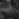
\includegraphics[height=2cm]{./imgs/B1_00005.png}

\section*{Gesichtserkennung und allgemeine Vorgehensweise}

Wir haben uns entschieden, Face Detection zu implementieren, da uns das Paper gut gefallen hat. Dabei haben wir
wie im Paper vorgeschlagen erstmal das Integralbild für je Beispiel berechnet und davon viele schwache Klassifizierer
erstellt, wobei je Klassifizier eine Form von den im Paper beschriebene haben kann und dazu noch beliebige Höhe,
Breite und Position. Dabei könnten wir noch mehr Positionen und Größen generieren, waren aber dabei ziemlich aufmerksam,
da das Performance bei mehreren Features drastisch senkt. Im Paper wurde vorgeschlagen, dazu noch mit beliebige Tresholds
auszuprobieren und das ganze als separate Klassifizierer zu betrachten. Wir haben aber lineare Regression genommen,
um von allen Werten, berechnet von allen Integralbilder und Features, möglichst schnell (beides Implementieraufwand und
Performance, einigermaßen) eine möglichst gute lineare Trennung zwischen den beiden Klassen anhand eines Werts zu
finden. Also unsere einzelne Klassifizierer sind lineare Regressionen, alle anhand von nur 1 Feature (z.B Differenz
zwischen die Helligkeit im linken und rechten Bereich des Bildes). \\ \\

Wir haben auch ausprobiert, bessere Ergebnisse zu bekommen, in dem wir eine Klasse mehr tolerieren.

\section*{Ergebnisse}

Wir haben mit unterschiedlichen Parameter das ganze ausprobiert. Dabei haben wir bemerkt, dass je mehr
Features und Klassifizierer man am Anfang generiert, desto bessere Ergebnisse man bekommt. Bei mehrere
ausgewählte Klassifizierer (nach AdaBoost) oder bei Tolerierung einer Klasse kann man schlecht was deutlich
besseres bekommen. Diesmal haben wir auch die Konfussionsmatrix benutzt, da wir oft ganz gute Fehlerrate bekommen
können, ohne echt gute Ergebnisse zu haben. Das ist so, da es deutlich mehrere Bilder ohne Gesichter im
Testdatensatz gibt, was dazu führt, dass man 30 Prozent Fehlerrate bekommen kann, wenn man immer die negative
Klasse vorhersagt. \\

Hier sind einige gute Beispiele (entweder relativ gute Ergebnisse oder ganz schlechte). Alle
Beispiele sind mit 2420 initiale Features bzw. Klassifizierer. \\

fp\_tolerate=0.3 (Wert zwischen 0 und 1 wie viel man die positive Klasse bevorzugt, später weiter erklärt) \\
60 Klassifizierer. Hier muss man aufpassen, dass wir prozentuell ganz gute Fehlerrate haben, aber kaum
welche Gesichter erkennen.

\begin{lstlisting}
2420 weak classifiers were successfully trained and their predictions saved!
Score train: 0.7556256270603411
Score test: 0.9167394468704513
Confusion matrix train:
[[4325 1482]
 [ 223  947]]
Confusion matrix test:
[[22032   461]
 [ 1541    11]]
\end{lstlisting}


fp\_tolerate=0.7, 300 Klassifizier
\begin{lstlisting}
2420 weak classifiers were successfully trained and their predictions saved!
Score train: 0.8251397448760213
Score test: 0.8468288625493866
Confusion matrix train:
[[4154  826]
 [ 394 1603]]
Confusion matrix test:
[[20234   344]
 [ 3339   128]]

\end{lstlisting}

Hier ist die Fehlerrate größer, die Ergebnisse sind aber deutlich besser, da man circa 84\% der Bilder ohne
Gesichter erkennt und dazu noch 37\% der Bilder mit Gesichter erkennt.

Es gibt noch 4 Beispiele in GitHub, die sind aber nicht zu interessant.


\section*{Evaluation}

Gesichtserkennung ist ein relativ schwieriges Entscheidungsproblem, deswegen sind unsere Ergebnisse auch nicht
perfekt. Wir haben aber bemerkt, dass AdaBoost eine ganz effektive und schnelle Methode ist. Die ist relativ
leicht einzustellen, man kann relativ leicht Klassen bevorzugen. Wenn man auch eine gute Menge von schwache
Klassifizierer hat, die anhand von total unteschiedliche Features funktionieren, kann man auch sehr gute
Ergebnisse bekommen. In unserem Fall, wenn man ganz simple Features benutzt, da man nicht sicher ist wie man mit
so ein Problem vorgehen kann, hat es auch super funktioniert. Das gute ist auch, dass wir mit dem Ansatz skalierbare
Klassifizerer benutzt haben und so alle Arten von Bilder und alle Größen von Gesichter erkennen können, ohne zu höhe
Laufzeitskosten.

\section*{Erklärung des Codes}
Diesmal werden wir nicht alles erklären, da das Code etwas mehr ist, man kann aber alles in GitHub finden.


\section*{Berechnung des Integralbilds}
Wir haben das Integralbild iterativ und nicht wie im Paper vorgeschlagen rekursiv berechnet,
da es uns auch in dem Fall intuitiver war. Hier ist row\_sum die Summe aller Pixeln über Position x.
Damit kann man die in den Integralimage gleich nach unten propagieren und mit dem Integralimage unten links
aufsummieren. So bearbeitet man das Bild von oben links nach unten rechts und pusht, so zu sagen, die Ergebnisse
immer nach unten.

\begin{lstlisting}[style=py]
def get_integral_image(img):
    row_sum = np.zeros(img.shape)
    integral_image = np.zeros((img.shape[0] + 1, img.shape[1] + 1), dtype=np.int64)

    for y, row in enumerate(img):
        for x, col in enumerate(row):
            row_sum[y, x] = row_sum[y - 1, x] + img[y, x]
            integral_image[y + 1, x + 1] = integral_image[y + 1, x] + row_sum[y, x]

    return integral_image
\end{lstlisting}

\section*{Berechnung der Summe innerhalb eines Rechtecks im Integralbild}

Die Vorgehensweise wurde sogar schon gegeben im Paper, nicht viel zu erklären hier. (Seite 140, Figure 3)
\begin{lstlisting}[style=py]
def get_integral_img_sub_sum(integral_image, top_left_position, bottom_right_position):
    top_left = top_left_position[1], top_left_position[0]
    bottom_right = bottom_right_position[1], bottom_right_position[0]

    if top_left == bottom_right:
        return integral_image[top_left]

    top_right = bottom_right[0], top_left[1]
    bottom_left = top_left[0], bottom_right[1]

    return np.int64(np.int64(integral_image[bottom_right]) - np.int64(integral_image[top_right]) -
                    np.int64(integral_image[bottom_left]) + np.int64(integral_image[top_left]))

\end{lstlisting}

\section*{Berechnung der Features}

Hier ist nur die Berechnung eines Features zu sehen, die Methode ist aber zeimlich lang und langweilig.
Hier ist nur interessant, dass wir Prozente für die Größe und Position für je Feature benutzt haben,
um das ganze skalierbar zu haben. Nachdem muss man nur alle notwendige Positionen auf dem Integralbild
berechnen und damit auch die Summen, nachher muss man nur das Endprodukt berechnen.

\begin{lstlisting}[style=py]
img_width = integral_image.shape[1] - 1
        img_height = integral_image.shape[0] - 1

        pos_x = int(self.xp * img_width)
        pos_y = int(self.yp * img_height)
        top_left = pos_x, pos_y

        br_x = int(pos_x + self.wp * img_width)
        br_y = int(pos_y + self.hp * img_height)
        bottom_right = br_x, br_y

        if self.type == FDFType.TWO_RECTANGLE_HORIZONTAL:
            middle_left = top_left[0], int(top_left[1] + self.hp * img_width / 2)
            middle_right = bottom_right[0], middle_left[1]
            a = get_integral_img_sub_sum(integral_image, top_left, middle_right)
            b = get_integral_img_sub_sum(integral_image, middle_left, bottom_right)

            return a - b
\end{lstlisting}

\section*{Generierung der Features}
Wie man hier sieht, könnten wir deutlich mehrere Positionen nehmen, war aber zu ineffizient.
\begin{lstlisting}[style=py]
        percents = np.arange(.4, .65, .05)
        # for a number of various feature positions, sizes and types,
        # create the pool of classifiers which will later be sieved with AdaBoost
        # Total amount of classifiers (features for face detection) is 405
        for wp in percents:
            for hp in percents:
                for xp in np.arange(0.1, 1 - wp, .1):
                    for yp in np.arange(0.1, 1 - hp, .1):
                        for f_type in types:
                            feature = FDFeature(wp, hp, f_type, xp, yp)
                            classifier = WeakClassifier(feature)
                            classifier_predictions.append(classifier.fit_predict(X_, y))
                            possible_classifiers.append(classifier)
\end{lstlisting}

\section*{Predict nach AdaBoost und damit Gesichtserkennung}
Wir haben bei der Berechnung von je Gewicht eines Klassifizierers die Teilung durch 2 weggelassen,
deswegen auch hier bei dem Vergleich mit der Summe aller Gewichten. Sonst ist alles wie im Paper.

\begin{lstlisting}[style=py]
    def predict(self, X):
        X_ = self.transform(X)
        predictions = np.zeros(len(X))

        for i, classifier in enumerate(self.classifiers):
            predictions += classifier.predict(X_) * self.cw[i]

        weights_sum = self.cw.sum()
        return np.vectorize(lambda p: 1 if p >= weights_sum else 0)(predictions)
\end{lstlisting}

\section*{AdaBoost}
Hier haben wir eher die im Tutorium vorgeschlagene Implementierung geguckt, aber das Paper war auch hilfreich.
Im Großen und Ganzen ist alles wie im Tutorium besprochen. Wir haben aber hier fp\_tolerate genommen, dass
bei der Initialisierung der Gewichte der einzelnen Beispiele helfen soll. Damit sollen erstmall die False Negatives
minimiert werden, wie man auch oben bei den Ergebnissen sieht. Die ganze Idee ist, dass man versucht eine Summe von
Gewicht 1 gleichmäßig erstmal zwischen den beiden Klassen und dann auch innerhalb einer Klasse zu verteilen. Mit
dem Parameter können wir aber definieren, dass eine Klasse, wie in dem Fall, 70\% aller Gewichte bekommen soll und
damit bevorzugt werden soll. Wie man in den Ergebnissen sieht, hat das funktioniert, aber eigentlich besser (zu
schlechtere deutlich Ergebnisse geführt) wenn man das falsch anwendet (fp\_tolerate = 0.3).

\begin{lstlisting}[style=py]
class AdaBoost:
    @staticmethod
    def boost_classifiers(classifier_pool, predictions, labels, k, fp_tolerate=0.7):
        data_size = len(labels)
        classifiers_count = len(classifier_pool)
        pos_size = len(labels[np.where(labels == 1)])
        neg_size = data_size - pos_size
        cw = []  # weights of chosen classifiers
        # initialize data set weights

        # here we take a slightly different approach from the general ada boost one
        # we have an fp_tolerate argument which can be set between 0 and 1
        # 0 fully ignores false positives and only tries to correct false negatives, 1 is opposite case
        # using this argument we can decide whether the error is equally separated between fp and fn
        data_weight = np.vectorize(lambda x: fp_tolerate / pos_size if x == 1 else (1 - fp_tolerate) / neg_size)(labels)
        classifiers = []

        # calculate error vector for each classifier
        # e.g. if a classifiers mistakes only 2. and 4. sample, its vector would be [0,1,0,1,0...,0]
        # that way, we can easily multiply the data-set weight vector by the error vector later on
        # to get e_i
        classifiers_e_vectors = np.zeros((classifiers_count, data_size), dtype=np.float64)
        for i in range(classifiers_count):
            wrong_idx = predictions[i] != labels
            # expected_pos = np.array(labels) == np.array([1] * len(labels))
            # false_negatives = np.logical_and(wrong_idx, expected_pos)
            # false_positives = np.invert(false_negatives)
            # wrongs = np.where(wrong_idx)

            classifiers_e_vectors[i][wrong_idx] = 1

        for j in range(k):
            e = classifiers_e_vectors.dot(data_weight) / data_weight.sum()
            idx_best = e.argmin()
            classifiers.append(classifier_pool[idx_best])

            e_i = e[idx_best]
            new_cw = np.log((1 - e_i) / (e_i + np.nextafter(0, 1)))
            cw.append(new_cw)

            signs = (classifiers_e_vectors[idx_best] - 0.5) * 2
            dw_update = np.vectorize(lambda s: np.exp(s * new_cw))(signs)
            data_weight = data_weight * dw_update

            classifier_pool = classifier_pool[:idx_best] + classifier_pool[idx_best + 1:]
            predictions = predictions[:idx_best] + predictions[idx_best + 1:]
            classifiers_e_vectors = np.delete(classifiers_e_vectors, idx_best, 0)

        return classifiers, np.array(cw)
\end{lstlisting}

\section*{Vollständiges Code}

\section*{AdaBoost.py}

\begin{lstlisting}[style=py]
import numpy as np


class AdaBoost:
    @staticmethod
    def boost_classifiers(classifier_pool, predictions, labels, k, fp_tolerate=0.7):
        data_size = len(labels)
        classifiers_count = len(classifier_pool)
        pos_size = len(labels[np.where(labels == 1)])
        neg_size = data_size - pos_size
        cw = []  # weights of chosen classifiers
        # initialize data set weights

        # here we take a slightly different approach from the general ada boost one
        # we have an fp_tolerate argument which can be set between 0 and 1
        # 0 fully ignores false positives and only tries to correct false negatives, 1 is opposite case
        # using this argument we can decide whether the error is equally separated between fp and fn
        data_weight = np.vectorize(lambda x: fp_tolerate / pos_size if x == 1 else (1 - fp_tolerate) / neg_size)(labels)
        classifiers = []

        # calculate error vector for each classifier
        # e.g. if a classifiers mistakes only 2. and 4. sample, its vector would be [0,1,0,1,0...,0]
        # that way, we can easily multiply the data-set weight vector by the error vector later on
        # to get e_i
        classifiers_e_vectors = np.zeros((classifiers_count, data_size), dtype=np.float64)
        for i in range(classifiers_count):
            wrong_idx = predictions[i] != labels
            # expected_pos = np.array(labels) == np.array([1] * len(labels))
            # false_negatives = np.logical_and(wrong_idx, expected_pos)
            # false_positives = np.invert(false_negatives)
            # wrongs = np.where(wrong_idx)

            classifiers_e_vectors[i][wrong_idx] = 1

        for j in range(k):
            e = classifiers_e_vectors.dot(data_weight) / data_weight.sum()
            idx_best = e.argmin()
            classifiers.append(classifier_pool[idx_best])

            e_i = e[idx_best]
            new_cw = np.log((1 - e_i) / (e_i + np.nextafter(0, 1)))
            cw.append(new_cw)

            signs = (classifiers_e_vectors[idx_best] - 0.5) * 2
            dw_update = np.vectorize(lambda s: np.exp(s * new_cw))(signs)
            data_weight = data_weight * dw_update

            classifier_pool = classifier_pool[:idx_best] + classifier_pool[idx_best + 1:]
            predictions = predictions[:idx_best] + predictions[idx_best + 1:]
            classifiers_e_vectors = np.delete(classifiers_e_vectors, idx_best, 0)

        return classifiers, np.array(cw)

\end{lstlisting}

\section*{FaceDetection.py}

\begin{lstlisting}[style=py]
import numpy as np
from Classifier import Classifier
from Parser import get_test_set, get_train_set
from Helpers import get_integral_image
from FDFeature import FDFeature
from FDFType import FDFType
from WeakClassifier import WeakClassifier
from AdaBoost import AdaBoost

types = [FDFType.TWO_RECTANGLE_HORIZONTAL, FDFType.TWO_RECTANGLE_VERTICAL,
         FDFType.THREE_RECTANGLE_HORIZONTAL, FDFType.THREE_RECTANGLE_VERTICAL,
         FDFType.FOUR_RECTANGLE]


class FaceDetection(Classifier):
    def __init__(self, k=300):
        self.classifiers = []
        self.cw = []  # classifier weights
        self.k_classifiers = k

    def fit(self, X, y):
        X_ = self.transform(X)

        # initialize all possible classifiers
        possible_classifiers = []
        classifier_predictions = []
        percents = np.arange(.4, .65, .05)

        # for a number of various feature positions, sizes and types,
        # create the pool of classifiers which will later be sieved with AdaBoost
        # Total amount of classifiers (features for face detection) is 405
        for wp in percents:
            for hp in percents:
                for xp in np.arange(0.1, 1 - wp, .1):
                    for yp in np.arange(0.1, 1 - hp, .1):
                        for f_type in types:
                            feature = FDFeature(wp, hp, f_type, xp, yp)
                            classifier = WeakClassifier(feature)
                            classifier_predictions.append(classifier.fit_predict(X_, y))
                            possible_classifiers.append(classifier)

        print('{} weak classifiers were successfully trained and their predictions saved!'.format(
            len(possible_classifiers)))

        self.classifiers, self.cw = AdaBoost.boost_classifiers(
            possible_classifiers, classifier_predictions, y, self.k_classifiers)

    def transform(self, X):
        return np.vectorize(lambda x: get_integral_image(x),
                            signature='(m,n)->(z,c)')(X)

    def predict(self, X):
        X_ = self.transform(X)
        predictions = np.zeros(len(X))

        for i, classifier in enumerate(self.classifiers):
            predictions += classifier.predict(X_) * self.cw[i]

        weights_sum = self.cw.sum()
        return np.vectorize(lambda p: 1 if p >= weights_sum else 0)(predictions)


X_test, y_test = get_test_set()
X_train, y_train = get_train_set()

ds_size = None
fd = FaceDetection()
fd.fit(X_train[:ds_size], y_train[:ds_size])
predictions_train = fd.predict(X_train[:ds_size])
predictions_test = fd.predict(X_test[:ds_size])
print('Score train: {}'.format(fd.score(predictions_train, y_train[:ds_size])))
print('Score test: {}'.format(fd.score(predictions_test, y_test[:ds_size])))
print('Confusion matrix train: \n{}'.format(fd.confusion_matrix(predictions_train, y_train[:ds_size])))
print('Confusion matrix test: \n{}'.format(fd.confusion_matrix(predictions_test, y_test[:ds_size])))

# print(X_test[0].shape)
#
# feature = FDFeature(.7, .3, FDFType.TWO_RECTANGLE_HORIZONTAL, .2, .2)
# wc = WeakClassifier(feature)
# X_train_ = np.vectorize(lambda x: get_integral_image(x),
#                         signature='(m,n)->(z,c)')(X_train)
# wc.fit(X_train_, y_train)
# print(wc.score(X_train_, y_train))

\end{lstlisting}

\section*{FDFeature.py}

\begin{lstlisting}[style=py]
from FDFType import FDFType
from Helpers import get_integral_img_sub_sum


class FDFeature:
    def __init__(self, width_percent, height_percent, type, pos_x_percent, pos_y_percent):
        self.wp = width_percent
        self.hp = height_percent
        self.type = type
        self.xp = pos_x_percent
        self.yp = pos_y_percent

    def get_value(self, integral_image):
        img_width = integral_image.shape[1] - 1
        img_height = integral_image.shape[0] - 1

        pos_x = int(self.xp * img_width)
        pos_y = int(self.yp * img_height)
        top_left = pos_x, pos_y

        br_x = int(pos_x + self.wp * img_width)
        br_y = int(pos_y + self.hp * img_height)
        bottom_right = br_x, br_y

        if self.type == FDFType.TWO_RECTANGLE_HORIZONTAL:
            middle_left = top_left[0], int(top_left[1] + self.hp * img_width / 2)
            middle_right = bottom_right[0], middle_left[1]
            a = get_integral_img_sub_sum(integral_image, top_left, middle_right)
            b = get_integral_img_sub_sum(integral_image, middle_left, bottom_right)

            return a - b
        elif self.type == FDFType.TWO_RECTANGLE_VERTICAL:
            middle_top = int(top_left[0] + img_width / 2 * self.wp), top_left[1]
            middle_bottom = middle_top[0], bottom_right[1]

            a = get_integral_img_sub_sum(integral_image, top_left, middle_bottom)
            b = get_integral_img_sub_sum(integral_image, middle_top, bottom_right)

            return a - b
        elif self.type == FDFType.THREE_RECTANGLE_HORIZONTAL:
            one_third_left = top_left[0], int(top_left[1] + 1 / 3 * img_height * self.hp)
            one_third_right = bottom_right[0], one_third_left[1]
            two_thirds_left = top_left[0], int(top_left[1] + 2 / 3 * img_height * self.hp)
            two_thirds_right = bottom_right[0], two_thirds_left[1]

            a = get_integral_img_sub_sum(integral_image, top_left, one_third_right)
            b = get_integral_img_sub_sum(integral_image, one_third_left, two_thirds_right)
            c = get_integral_img_sub_sum(integral_image, two_thirds_left, bottom_right)

            return a - b + c
        elif self.type == FDFType.THREE_RECTANGLE_VERTICAL:
            one_third_top = int(top_left[0] + 1 / 3 * self.wp * img_width), top_left[1]
            one_third_bottom = one_third_top[0], bottom_right[1]
            two_thirds_top = int(top_left[0] + 2 / 3 * self.wp * img_width), top_left[1]
            two_thirds_bottom = two_thirds_top[0], bottom_right[1]

            a = get_integral_img_sub_sum(integral_image, top_left, one_third_bottom)
            b = get_integral_img_sub_sum(integral_image, one_third_top, two_thirds_bottom)
            c = get_integral_img_sub_sum(integral_image, two_thirds_top, bottom_right)

            return a - b + c
        elif self.type == FDFType.FOUR_RECTANGLE:
            middle_left = top_left[0], int(top_left[1] + self.hp * img_width / 2)
            middle_right = bottom_right[0], middle_left[1]
            middle_top = int(top_left[0] + img_width / 2 * self.wp), top_left[1]
            middle_bottom = middle_top[0], bottom_right[1]
            middle = middle_top[0], middle_left[1]

            a = get_integral_img_sub_sum(integral_image, top_left, middle)
            b = get_integral_img_sub_sum(integral_image, middle_top, middle_right)
            c = get_integral_img_sub_sum(integral_image, middle_left, middle_bottom)
            d = get_integral_img_sub_sum(integral_image, middle, bottom_right)

            return (a + d) - (b + c)

        return 0

\end{lstlisting}

\section*{FDFType.py}

\begin{lstlisting}[style=py]
from enum import Enum


class FDFType(Enum):
    TWO_RECTANGLE_HORIZONTAL = 1
    TWO_RECTANGLE_VERTICAL = 2
    THREE_RECTANGLE_HORIZONTAL = 3
    THREE_RECTANGLE_VERTICAL = 4

    # it makes no sense to differ between horizontal and vertical here
    # as it is the difference between the diagonals
    # positive or negative, it is the same number, we don't really care
    FOUR_RECTANGLE = 5

\end{lstlisting}

\section*{WeakClassifier.py}

\begin{lstlisting}[style=py]
from sklearn.linear_model import LinearRegression
import numpy as np
from Classifier import Classifier

class WeakClassifier(Classifier):
    def __init__(self, feature):
        self.feature = feature
        self.lr = LinearRegression()

    def fit(self, X, y):
        X_ = self.transform(X)
        y_ = np.vectorize(lambda x: 1 if x == 1 else -1)(y)
        self.lr.fit(X_, y_)

    def fit_(self, X, y):
        self.lr.fit(X, y)

    def fit_predict(self, X, y):
        X_ = self.transform(X)
        y_ = np.vectorize(lambda x: 1 if x == 1 else -1)(y)
        self.fit_(X_, y_)
        return self.predict_(X_)

    def predict(self, X):
        X_ = self.transform(X)
        return self.predict_(X_)

    def predict_(self, X):
        predictions = self.lr.predict(X)
        return np.vectorize(lambda x: 1 if x > 0 else 0)(predictions)

    def transform(self, X):
        return np.vectorize(lambda x: self.feature.get_value(x),
                            signature='(m,n)->()')(X).reshape(-1,1)


\end{lstlisting}

\section*{Helpers.py}

\begin{lstlisting}[style=py]
import numpy as np


def get_integral_image(img):
    row_sum = np.zeros(img.shape)
    integral_image = np.zeros((img.shape[0] + 1, img.shape[1] + 1), dtype=np.int64)

    for y, row in enumerate(img):
        for x, col in enumerate(row):
            row_sum[y, x] = row_sum[y - 1, x] + img[y, x]
            integral_image[y + 1, x + 1] = integral_image[y + 1, x - 1 + 1] + row_sum[y, x]

    return integral_image


def get_integral_img_sub_sum(integral_image, top_left_position, bottom_right_position):
    # as x and y coordinates in an image are flipped, therefore they are flipped within the integral image as well
    # as you can see in the upper method, we take the rows as y and cols as x, but in the final result we leave
    # them as they are

    top_left = top_left_position[1], top_left_position[0]
    bottom_right = bottom_right_position[1], bottom_right_position[0]

    # sum of a single cell, as coords of top left and bottom right corner of sub-image are identical
    if top_left == bottom_right:
        return integral_image[top_left]

    top_right = bottom_right[0], top_left[1]
    bottom_left = top_left[0], bottom_right[1]

    return np.int64(np.int64(integral_image[bottom_right]) - np.int64(integral_image[top_right]) -
                    np.int64(integral_image[bottom_left]) + np.int64(integral_image[top_left]))

\end{lstlisting}

\section*{Parser.py}

\begin{lstlisting}[style=py]
import numpy as np
import glob
import os
import cv2

def read_pgm(file_name):
    return cv2.imread(file_name, -1)


def get_data_set(data_set_type='test'):
    data_folder = os.path.abspath(os.path.join(os.path.dirname(__file__), './Dataset'))
    faces = glob.glob(data_folder + '/{}/face/*.pgm'.format(data_set_type))
    non_faces = glob.glob(data_folder + '/{}/non-face/*.pgm'.format(data_set_type))
    data_set = []
    labels = []

    for file in faces:
        image = read_pgm(file)
        data_set.append(image)

    for file in non_faces:
        image = read_pgm(file)
        data_set.append(image)

    labels = labels + ([1]*len(faces))
    labels = labels + ([0]*len(non_faces))
    labels = np.array(labels)

    data_set = np.array(data_set)
    np.random.seed(1)
    idx = np.random.permutation(len(data_set))

    # return a random permutation so positive and negative samples are mixed
    return data_set[idx], labels[idx]


def get_test_set():
    return get_data_set('test')


def get_train_set():
    return get_data_set('train')

\end{lstlisting}
% /////////////////////// END DOKUMENT /////////////////////////
\end{document}
